\subsection{Non-Dynamic GNN Explanation}
Explainability in dynamic graph neural networks can be challenging due to the complex and non-linear nature of GNN models. However, using non-machine learning techniques or interpretable-by-design machine learning techniques can be a reasonable approach depending on problem-specific requirements. Figure \ref{fig:avoiding-dgnn-diagram} shows a decision tree of these possible alternatives.

\textbf{Non-machine learning techniques} like rule-based systems, Arima, DTW or decision trees, often provide explicit rules, similarities or decision paths that can be easily understood and interpreted. These less complex techniques benefit from lighter computational requirements and can offer more interpretability. Moreover, machine learning is only predictive if the training examples are similar to the predicted examples. This means new or unlearned patterns will go undetected. The EvolveGCN\cite{pareja_evolvegcn_2019} displays the inaccuracies in bitcoin transaction classification using machine learning techniques when faced with a black swan event: a sudden underground market taken offline. This is illustrated in Figure \ref{fig:elliptic-fraud-f1} with elliptic dataset, discussed further in the Discussion section. Despite these benefits, non-machine learning techniques may not fully capture the complex hidden relationships in dynamic graphs as effectively as GNNs, illustrating the trade-off between obtaining additional accuracy and sacrificing interpretability for explainability.

The accuracy-interpretability trade-off is fundamental in machine learning: as the complexity of the model increases, interpretability tends to decrease and vice versa. Machine learning models like GNNs take this interpretability trade-off to the extreme; as soon as you implement a machine learning model, you sacrifice all interpretability and are forced to add additional abstracted explainers to try and recoup the lost understanding. GNNs illustrate this by achieving higher accuracy by better capturing graph relationships at the expense of interpretability.

\begin{figure}
    \centering 
    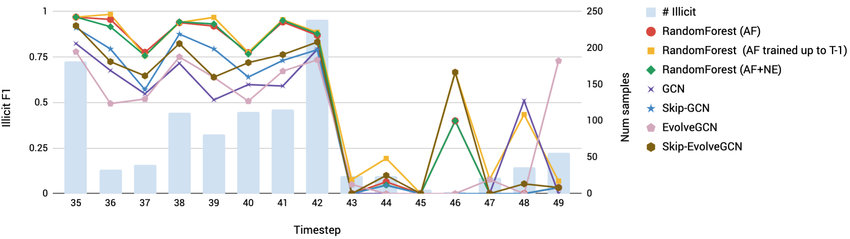
\includegraphics[width=\textwidth]{images/elliptic-fraud-f1.png}
    \caption{F1 evolution facing a crash in the elliptic dataset. At time t=43, the sudden disappearance of a Dark Market has a notable adverse impact on the performance of all models in subsequent periods.\cite{bellei_elliptic_2019}}
    \label{fig:elliptic-fraud-f1}
\end{figure}

\textbf{Classical machine learning techniques} like support vector machines (SVMs), XGBoost, or random forests can also provide some form of interpretability. These models are generally easier to understand and provide insights into the importance of different graph features. Including graph features enrichment can even improve the accuracy of classical models to a level comparable to GNNs\cite{rao_modelling_2022}! Graph feature enrichment involves extracting meaningful features (e.g., neighborhood information) from the graph structure to enhance the predictive power of the model.

\begin{figure}
    \centering 
    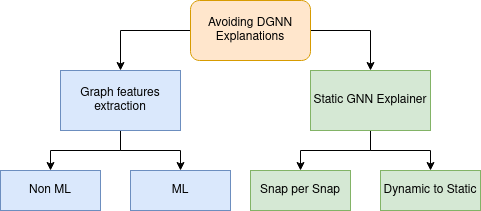
\includegraphics[width=0.75\textwidth]{images/avoiding-dgnn-diagram.png}
    \caption{Avoiding dynamic GNN explainers}
    \label{fig:avoiding-dgnn-diagram}
\end{figure}

A different, counter-intuitive alternative to using dynamic GNN explainers is modifying static GNN explainers. There are two ways to adapt them:

\textbf{Snapshot-per-snapshot explanation} involves providing explanations for each snapshot of the dynamic graph individually, without considering time evolution. By focusing on each snapshot independently, this method is simple and provides explanations that are specific to the features and relationships within that particular snapshot. This has one main limitation: \textit{losing temporal context}. Dynamic graphs often have time-dependent patterns and relationships that can influence the behavior of the network, leading to incomplete or misleading explanations. Despite this, we argue that static GNN explainers may be a good fit for a temporal GNN in many scenarios.

\textbf{Transforming dynamic graphs into a static graph} involves augmenting the dynamic graph by adding temporal edges, effectively transforming it into a static graph\cite{kim_temporal_2022}. By adding temporal edges, the transformed static graph retains the temporal relationships between different snapshots. This allows for the utilization of traditional static GNN explainers while still considering the time evolution of graphs. These explanations can then reflect the influence of temporal dependencies on the GNN's behavior. However, transforming a dynamic graph into a static graph by adding temporal edges introduces additional complexity. Pruning the graph and modifying the explainer to each specialized static graph might be necessary. We found no papers on this topic, but we expect it to be a topic in future research.

The choice between each of the two static GNN explainer methods depends on the target problem, importance of temporal context, and trade-off between simplicity and capturing temporal dynamics.

\subsection{Dynamic GNN explanation}
Table \ref{table-3-full} was already introduced in section 2.4, but we include further details on the papers here. These papers try to combine the best of both machine learning accuracy and and a human understandable model-decision process.
\begin{itemize}
    \item STpGCN\cite{ye_explainable_2023} captures the spatial-temporal graph representation of brain activities by incorporating multi-scale temporal dependency via graph structures. In addition, the paper introduces a sensitivity analysis method called BrainNetX, which automatically annotates task-related brain regions from a brain-network standpoint, enhancing the explainability of decoded results while validating the hierarchical structure of STpGCN.
    \item TGNNExplainer\cite{he_explainer_2022} framework consists of two modules: the first module explains each time step prediction independently using a probabilistic graphical model, and the second module discovers the dominant interesting explanations in a time period.
    \item DGExplainer\cite{xie_explaining_2022} redistributes the output activation scores of a dynamic GNN to the neurons in its previous layer, creating input neuron relevance scores. The input relevance explains the model decision.
    \item XHGP\cite{limeros_towards_2022} utilizes GNNExplainer, attention, and counterfactual reasoning to improve the prediction explanations. The model is being developed for autonomous vehicles, with its graph and challenges unique to that field.
    \item GCN-SE\cite{fan_gcn-se_2021} uses squeeze and excitation to find snapshot attention weights, illustrating the predictive power of attention interpretability.
    \item RNN-GCN\cite{yao_interpretable_2021} weights each edge based on its longevity. A decay rate is used to lower edge importance as time goes on. An optimal decay is calculated for each cluster and is interpreted as importance of historical connection information.
    \item FraudMemory\cite{yang_fraudmemory_2019} computes three fraud scores: sequential, group, and individual fraud score. FraudMemory merges them to make a final prediction. The three scores can each be viewed as a  potential source of anomalies. The subscores also contribute to both model decisions and interpretation of fraudulent behavior.
\end{itemize}

Certain dynamic graph neural networks (GNNs) employ attention mechanisms, decay rates, or sub-scores to enhance interpretability. While interpretability is advantageous due to its inherent transparency without requiring a post-hoc explainer, it has limitations and cannot, for instance, calculate feature importance\cite{yao_interpretable_2021}. Therefore, interpretability and explainability should be regarded as complementary aspects rather than substitutes. If a higher level of transparency and comprehension of the model is desired, dynamic explainers can be employed on top of an interpretable GNN.

\clearpage
\begin{figure}
    \centering
    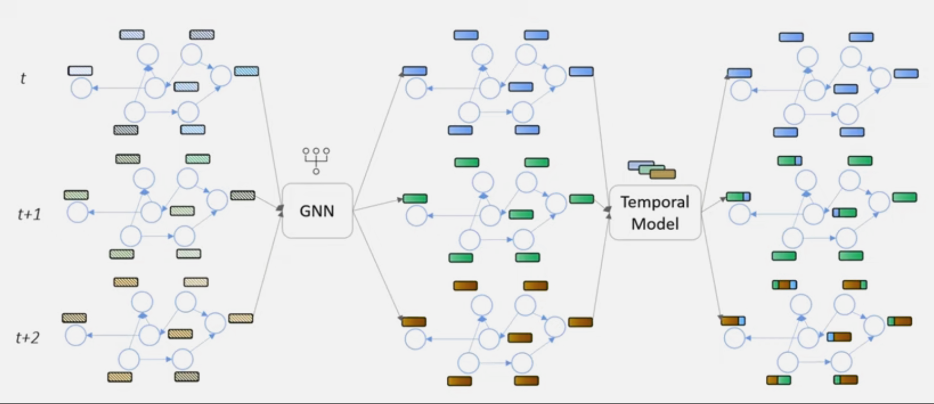
\includegraphics[width=\textwidth]{images/tgn-embedding-white.png}
    \caption{TGN and Spacio-temporal embeddings \cite{deepfindr_friendly_2021}. The raw snapshots on the left side are subjected to processing by a static GNN. In the middle, the snapshots incorporate spatial information as a result of message passing and aggregation. On the right side, the static spatial information of each node is combined over time to create a spatio-temporal embedding. In other words, previous embeddings are used as node history.}
    \label{fig:tgn-embedding}
\end{figure}

Using only a slightly-modified GNN explainer in specific contexts can produce striking results:
\begin{enumerate}
    \item Consider that gradient, surrogate, perturbation and decomposition methods can be used for dynamic GNNs in the same way they would normally used for static graphs. This is possible because node embeddings contain \textit{all} necessary temporal information. Apply one of these methods to a dynamic graph dataset.
    \item Continue by attaching an GNN explainer to this model that processes each snapshot individually.
    \item Aggregate the node embeddings, and collect the result.
\end{enumerate}

This is the process illustrated in figure \ref{fig:tgn-embedding}. All the temporal, spatial and feature information is being gathered on the embeddings in the bottom-right corner of the figure. A static explainer is able to perfectly explain the importance of each part of these embeddings; this implies that dynamic explainers are not needed for models that combine all information into one embedding. This is significant because this is practice for graphs where nodes don't appear or disappear often. The need for dynamic specific explainability is therefore mostly limited to dynamic graphs that strongly vary over time.